
With increased precision of data, the calculations must also progress to higher accuracy, involving an increased number of diagrams with each 
additional order, and this translates into computationally demanding 
calculations even for the DIS processes. Such calculations 
are too slow to be used iteratively in a fit.
There are several methods available which allow fast PDF extractions.  
Two such techniques
are implemented into \fitter\ : the $k-factor$ approximation from lower (LO) to higher order (NLO) and the fast grid techniques using interfaces to the 
packages FastNLO and APPLGRID. These techniques are briefly described below.  


\begin{description}
\item \bf {$k-factor$ technique:} \rm

A $k-factor$ is a ratio of the prediction between a high-order (slow)
pQCD calculation and the lowest-order (fast) calculation.  These `` k-factors''
are evaluated as a function of the kinematic variables relevant to
 the measurement 
for a fixed PDF (for example the first iteration of the fit) and stored in 
tables. They can then be applied 'on the fly' to each subsequent fit 
iteration which will use the fast prediction multiplied by this `` k-factor''.
Having determined a PDF this way the output PDF fit should then be used to 
recalculate the k-factors and the fit repeated until input and output 
$k-factors$ have converged. 

\begin{itemize}
\item For the DIS process, the heavy flavour schemes provide accurate but computationally slow calculations. In \fitter `` FAST'' schemes were implemented 
such that the $k-factor$ used can be
the ratio between same order calculations but massless vs massive 
(i.e. NLO (ZM-VFNS)/NLO (ACOT), or 
the ratio between LO (massless)/NLO (massive).
The $k-factors$ are only calculated for the PDF parameters at the first 
fit iteration
 and hence, the FAST heavy flavour schemes should only be used 
for quick checks and the full scheme is recommended.
%Hence the RT-fast calculation must be repeated by inputting the final PDF parameters 
%and iterating this procedure until the input and output PDFs are not significantly different
%%%%
The method was employed in the QCD fits to the HERA data when ACOT scheme was used as a cross check of the central results \cite{h1zeus:2009wt}, as shown in Fig.~\ref{fig:acotrt}.
\begin{figure}[!ht]
   \centering
   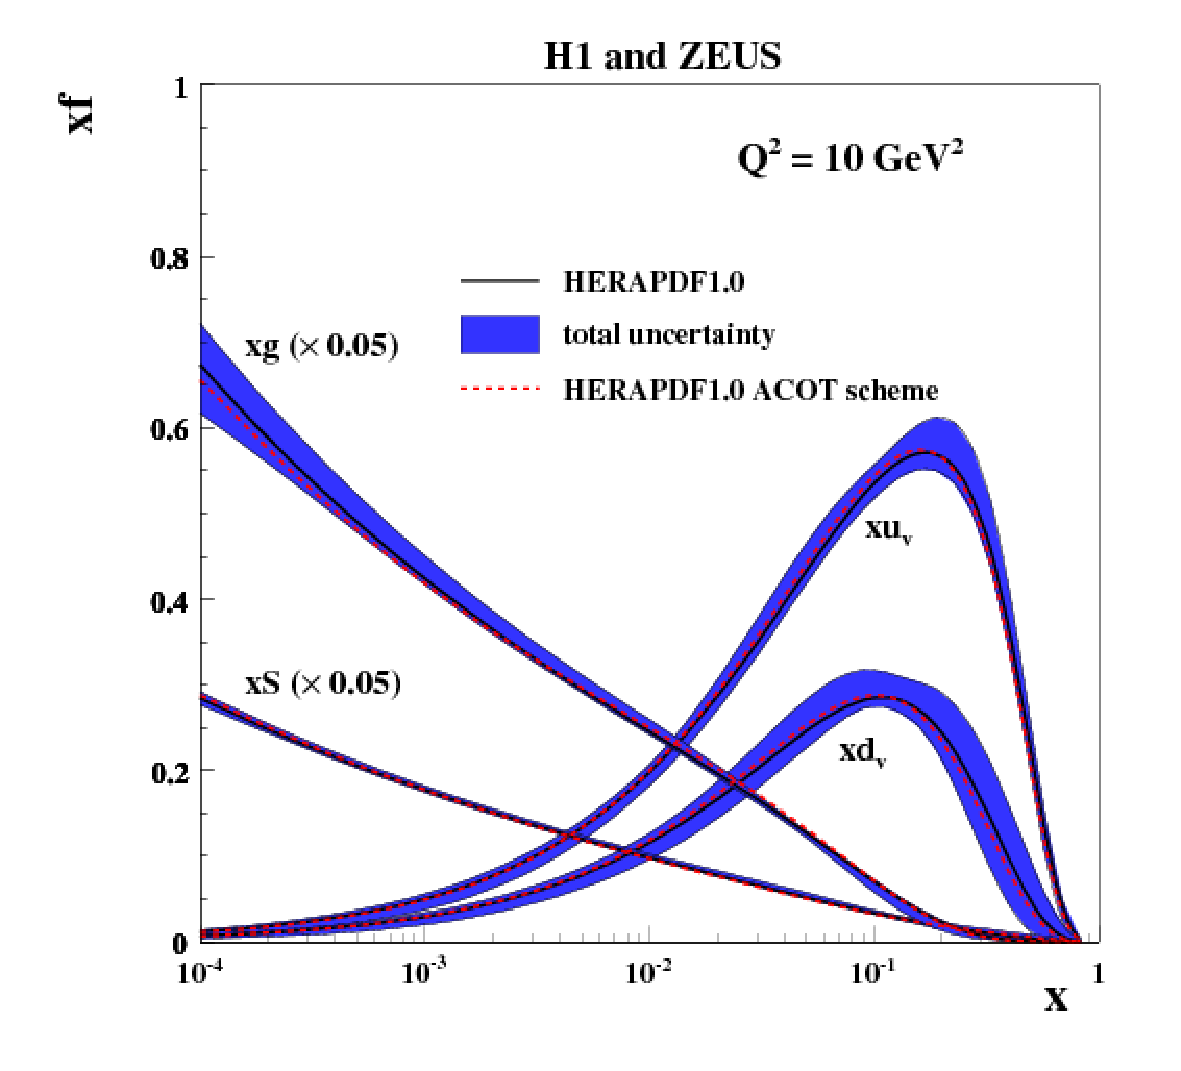
\includegraphics[width=8cm]{heraacot.pdf}
   \caption{Summary plots of valence, total sea (scaled) and gluon (scaled)densities with their total model uncertainties at the scale of $Q^2=10$ Gev$^2$ obatined using ACOT scheme with $k-factor$ method (red) compared to the HERAPDF1.0 PDF set at NLO using RT scheme.}
 \label{fig:acotrt}
\end{figure}



\item 
In the case of the DY processes the LO calculation described in section~\ref{dysection}
is such that the PDF functions factorise, allowing high speed calculations when 
performing parameter fits over lepton rapidity data. In this case
the factorised part of the expression which is independent of PDFs can be
calculated only once for all minimisation iterations.
The leading order code in \fitter\ package implements this 
optimisation and uses fast convolution routines provided by
QCDNUM. Currently the full width LO calculations are optimised 
for lepton pseudorapidity and boson rapidity distributions with the
possibility to apply lepton \(p_{\perp}\) cuts.
%making this procedure flexible to describe data.
This flexibility allows the calculations to be performed within the phase space
corresponding to the available measurement.

%The calculated leading order cross sections are multiplied by
%NLO or NNLO k-factors provided for corresponding data distributions.
The calculated leading order cross sections are multiplied by
$k-factors$ to obtain predictions at NLO.

\end{itemize}

%or NNLO precision.
%%%%
%\subsubsection{APPLGRID}
%\vspace{0.1cm}


\item \bf {Fast Grid Techniques:} \rm


\begin{itemize}
\item The APPLGRID~\cite{Carli:2010rw} package allows the fast computation 
of NLO cross sections for particular processes for arbitrary sets of 
proton parton distribution functions. The package implements
calculations of DY production as well as jet production in $pp(\bar p)$
collisions and DIS processes. 

The approach is based on storing the perturbative coefficients
of NLO QCD calculations of final-state observables measured
in hadron colliders in look-up tables. The PDFs and the 
strong couplings are included during the final calculations,
e.g. during PDF fitting. The method allows 
variation of factorization and renormalization scales in
calculations.

The look-up tables (grids) can be generated with modified versions
of the MCFM parton level generator for DY~\cite{Campbell:1999ah,Campbell:2000je,Campbell:2010ff} 
or NLOjet++~\cite{Nagy:1998bb,Nagy:2001fj} code for NLO jet production.
The model input parameters are pre-set as usual for MCFM, 
while binning and definitions of the
cross section observables are set in the APPLGRID code.
%as distributed with the full version of APPLGRID package.
% NLO calculations
%for the current analysis are performed with the help of APPLGRID
%generated grids based on MCFM calculations. 
%
%APPLGRID supports an interface to the MCFM parton level generators,
%hence model input parameters such as electroweak parameters
%are in fact pre-set following the MCFM input steering card, while
%binning and definitions of the observables for which the
%differential cross sections are needed are set in the 
%APPLGRID code. 
%The grid parameters \(x_1, x_2\) and \(Q^2\) binning
The grid parameters, \(Q^2\) binning
and interpolation orders are also defined in the code.

APPLGRID constructs the grid tables in two 
steps: {\it (i)} exploration of the phase space in order
to optimize the memory storage and {\it (ii)} actual grid
construction in the phase space corresponding to the 
requested observables.
The NLO cross sections are restored from the grids
using externally provided PDFs, \(\alpha_S\), factorization and 
renormalization scales. For NNLO predictions $k-factors$ can be applied.

This method was used by the ATLAS collaboration in determining the strange 
quark density of the proton from $W$ and $Z$ cross sections~\cite{atlas:strange}. 
An illustration of ATLAS PDFs extracted using $k-factor$ method is shown 
in Fig.~\ref{fig:atlas} togehter with the comparison to global PDF sets 
CT10~\cite{CT10pdf} and NNPDF2.1~\cite{NNPDFpdf}.

\begin{figure}[!ht]
   \centering
   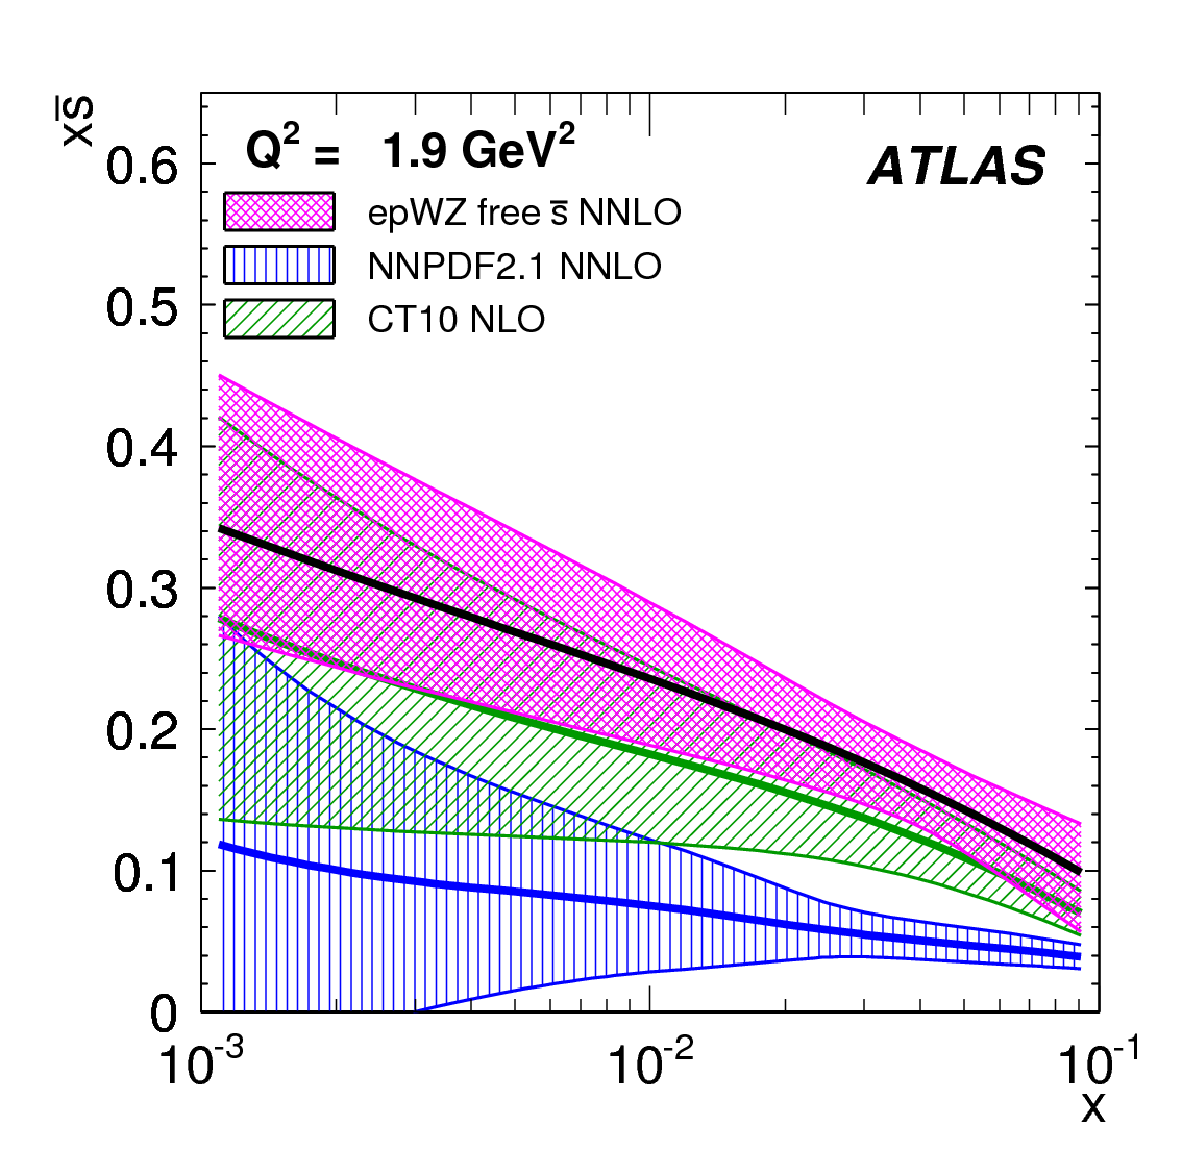
\includegraphics[width=8cm]{atlas.pdf}
   \caption{The strange anti-quark density versus $x$ for the ATLAS epWZ free sbar NNLO fit (magenta band) compared to predictions from NNPDF2.1 (blue hatched) and CT10 (green hatched) at $Q^2= 1.9$ GeV$^2$.}
 \label{fig:atlas}
\end{figure}


\item
The FastNLO project~\cite{Kluge:2006xs,Wobisch:2011ij,Britzger:2012bs}
%enables the inclusion of jet data in PDF and $\alpha_s$ fits.
uses multi-dimensional interpolation
techniques to convert the convolutions of perturbative 
coefficients with parton distribution functions and 
the strong coupling into simple products.
%Although the concept is process independent, 
The perturbative 
coefficients are calculated by the \texttt{NLOJET++}
program~\cite{Nagy:1998bb} where, 
in addition to the jet production processes available in MCFM,
calculations for jet-production
in DIS~\cite{Nagy:2001xb} are available as well as calculations for 
hadron-hadron 
collisions~\cite{Nagy:2003tz,Nagy:2001fj} which include
 threshold-corrections 
at $\mathcal{O}$(NNLO) for inclusive jet cross 
sections~\cite{Kidonakis:2000gi}.

The fastNLO libraries are included in the \fitter\ package.
%and no further requirements or compilation options
%are needed.
In order to include a new measurement into the PDF fit,
the fastNLO tables have to be specified. These tables include all
necessary information about the perturbative coefficients and the
calculated process for all bins of a certain dataset. 
%Tables for almost all published jet measurements
%are available through the project website \\ {\tt http://fastnlo.hepforge.org}.
%
%Features of the fastNLO concept are the very quick convolution of the
%perturbative coefficients with the PDFs, of
%$\mathcal{O}(100 ms)$, and the very high accuracy
%of the interpolation procedure. 
The fastNLO tables were originally calculated
for multiple factors of the factorization scale, 
and a renormalization scale factor could be chosen freely.
More recently, some of the fastNLO tables allow for 
%already involve a scale-independent
%concept~\cite{Britzger:2012bs}, which allows for 
the free choice~\cite{Britzger:2012bs} of the renormalization and the factorization
scale as a function of two pre-defined observables.
The evaluation of the strong coupling constant, which enters
the cross section calculation, is taken consistently from the 
QCDNUM evolution code.

The fastNLO methodology were used in the recent CMS analysis with \fitter where the impact
on the extraction of the PDFs from the inclusive jet cross section is investigated~\cite{cms:jets}. 
The impact of the gluon density of CMS inclusive jet data is illustrated in Fig.~\ref{fig:cmsjet}.
\begin{figure}[!ht]
   \centering
   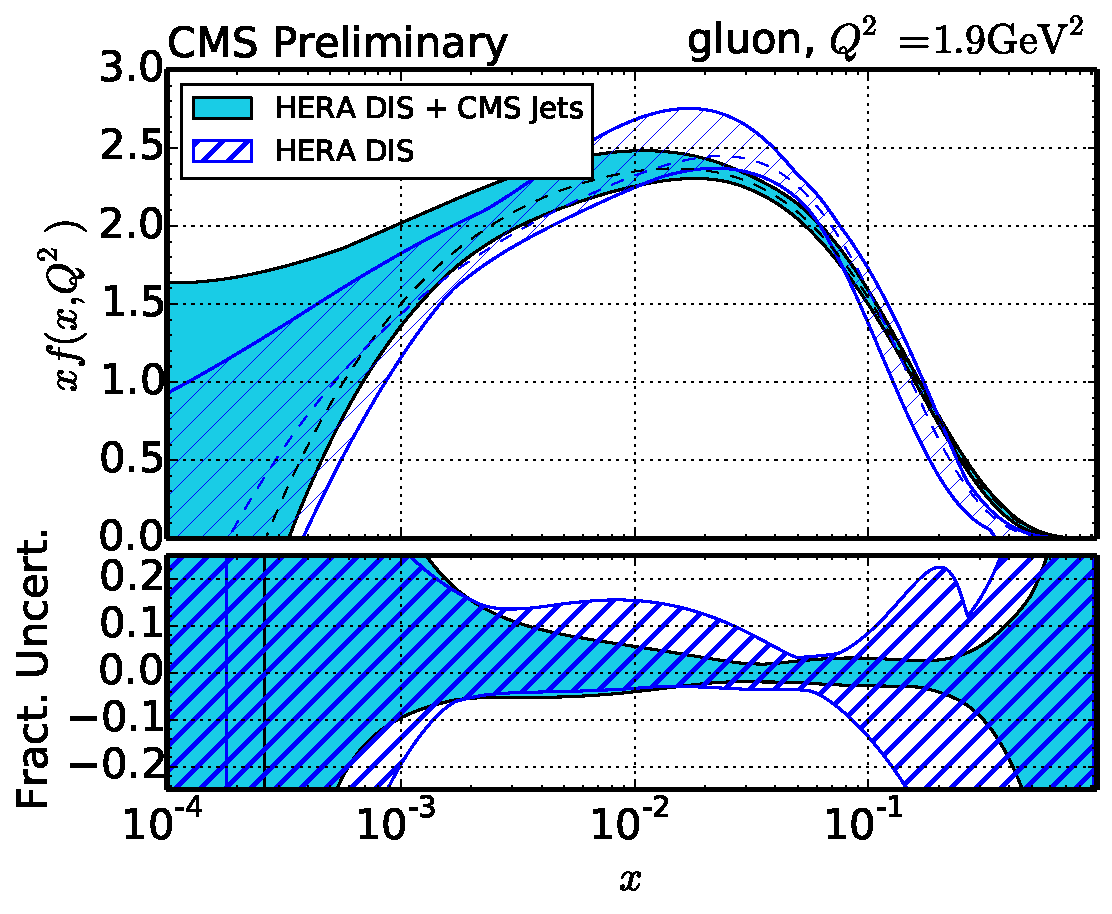
\includegraphics[width=8cm]{CMSjets.pdf}
   \caption{The gluon density as a function of $x$ as derived from HERA inclusive DIS data 
            alone (cyan) and in combination with CMS inclusive jet data from 2011 (blue hatched)
            where bands represent the total uncertainty of the PDFs. 
            The PDFs are shown at the starting scale $Q^2= 1.9$ GeV$^2$.}
 \label{fig:cmsjet}
\end{figure}


\end{itemize}

\end{description}

